# RUP: Rational Unified Process

## ¿Qué es y para qué sirve?

### ¿Qué es y para qué sirve?

\bld{Definición concreta}:

\begin{rboxx}{}
\texthigh{Rational Unified Process (RUP):}\\
es una metodología aplicable al proceso de desarrollo de \itt{software}
\end{rboxx}

- Fue desarrollada por la empresa ``Rational Software''.
    - La cual ahora pertenece a IBM.

## Características

### Características

\begin{center}
\begin{tiny}
\smartdiagramanimated[constellation diagram]{
    RUP,Guiado por\\casos de uso,Centrado\\en la\\arquitectura,Iterativo e\\incremental,Desarrollo\\basado en\\componentes,Utiliza UML,Proceso integrado}
\end{tiny}
\end{center}

### Estructura

- RUP está estructurado en \texthigh{fases} y \texthigh{disciplinas} (componentes).
- Se suele ilustrar mediante el diagrama ``RUP hump'' \footnote{Imagen obtenida desde \url{http://www.ibm.com/developerworks/rational/library/feb05/krebs}}:

\vfill

\centering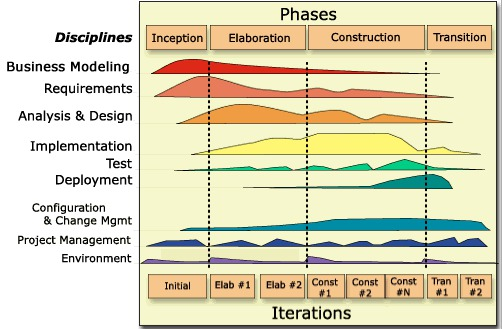
\includegraphics[width=.6\textwidth]{img/rup-ibm-phases.jpg}


## Estructura

### Estructura: Fases

Las \texthigh{fases} corresponden a la división temporal del proceso:

\vfill

\buildrboxx{}

1. Inicio o gestación (\itt{Inception}).
1. Elaboración (\itt{Elaboration}).
1. Construcción (\itt{Construction}).
1. Transición (\itt{Transition}).

\finishrboxx

\vfill

\def\distFlow{1em}
\begin{center}\begin{tikzflowchart}
  \node (a1) [flow1] {Inicio};
  \node (a2) [flow2, right=\distFlow of a1] {Elaboración};
  \node (a3) [flow3, right=\distFlow of a2] {Construcción};
  \node (a4) [flow4, right=\distFlow of a3] {Transición};
  \draw[arrow] (a1) -- (a2);
  \draw[arrow] (a2) -- (a3);
  \draw[arrow] (a3) -- (a4);
\end{tikzflowchart}\end{center}

### Fase de Inicio

\def\distFlow{1em}
\begin{center}\begin{tikzflowchart}
  \node (a1) [flow1] {Inicio};
  \node (a2) [flow0, right=\distFlow of a1] {Elaboración};
  \node (a3) [flow0, right=\distFlow of a2] {Construcción};
  \node (a4) [flow0, right=\distFlow of a3] {Transición};
  \draw[arrow] (a1) -- (a2);
  \draw[arrow] (a2) -- (a3);
  \draw[arrow] (a3) -- (a4);
\end{tikzflowchart}\end{center}

\vfill

- Se establece la \texthigh{oportunidad} y el \texthigh{alcance} del proyecto.
- Se identifica todas las entidades externas involucradas (\texthigh{actores}).
- Se define la \texthigh{interacción a un alto nivel de abstracción}:
    - Se identifica todos los casos de uso.
    - Algunos de ellos son descritos en detalle.

\vfill

- La \texthigh{oportunidad del negocio} analizado incluye:
    - Criterios de éxito.
    - Identificación de riesgos.
    - Estimación de recursos necesarios.
    - Plan de las fases, incluyendo hitos.

### Fase de Inicio

\def\distFlow{1em}
\begin{center}\begin{tikzflowchart}
  \node (a1) [flow1] {Inicio};
  \node (a2) [flow0, right=\distFlow of a1] {Elaboración};
  \node (a3) [flow0, right=\distFlow of a2] {Construcción};
  \node (a4) [flow0, right=\distFlow of a3] {Transición};
  \draw[arrow] (a1) -- (a2);
  \draw[arrow] (a2) -- (a3);
  \draw[arrow] (a3) -- (a4);
\end{tikzflowchart}\end{center}

Los \texthigh{productos} generados en esta etapa son:
\vfill

- Documento de visión general.
    - Requisitos generales del proyecto.
    - Características principales.
    - Restricciones.
\vfill
- Modelo inicial de casos de uso.
    - Un 10\% a un 20\% ya listos.
\vfill

- Identificación inicial de riesgos.
\vfill

- Plan del proyecto.
\vfill

- Uno o más prototipos.

### Fase de Inicio

- El término de esta fase constituye un hito:

\def\distFlow{1em}
\def\distMilestone{2em}
\begin{center}\begin{tikzflowchart}
  \node (a1) [flow1] {Inicio};
  \node (a2) [flow0, right=\distFlow of a1] {Elaboración};
  \node (a3) [flow0, right=\distFlow of a2] {Construcción};
  \node (a4) [flow0, right=\distFlow of a3] {Transición};
  \draw[arrow] (a1) -- (a2) node[midway,below] (nn1) {};
  \draw[arrow] (a2) -- (a3);
  \draw[arrow] (a3) -- (a4);
  \node (nn2) [below=\distMilestone of nn1, color=red] {Objetivos del ciclo de vida};
  \draw[arrow] (nn2) -- (nn1);
\end{tikzflowchart}\end{center}

- En este momento las partes interesadas deben acordar el alcance y la estimación de tiempo y costo.
- Se deben comprender los requisitos expresados en los casos de uso.
\vfill

- Si esto \textcolor{red}{no se cumple}:
    - El proyecto se cancela o esta etapa se repite.

### Fase de Elaboración

\def\distFlow{1em}
\begin{center}\begin{tikzflowchart}
  \node (a1) [flow0] {Inicio};
  \node (a2) [flow2, right=\distFlow of a1] {Elaboración};
  \node (a3) [flow0, right=\distFlow of a2] {Construcción};
  \node (a4) [flow0, right=\distFlow of a3] {Transición};
  \draw[arrow] (a1) -- (a2);
  \draw[arrow] (a2) -- (a3);
  \draw[arrow] (a3) -- (a4);
\end{tikzflowchart}\end{center}

\begin{rboxx}{}
Esta es la etapa donde el proyecto comienza a tomar forma.
\end{rboxx}

\bld{Objetivo principal:}

- \texthigh{Eliminar o mitigar} los elementos de mayor \texthigh{riesgo} para el desarrollo del proyecto.
    - Estos riesgos ya fueron identificados en la fase de inicio.

\bld{Objetivos secundarios:}

- Analizar el \texthigh{dominio} del problema.
- Establecer una \texthigh{arquitectura} base sólida.

### Fase de Elaboración

\def\distFlow{1em}
\begin{center}\begin{tikzflowchart}
  \node (a1) [flow0] {Inicio};
  \node (a2) [flow2, right=\distFlow of a1] {Elaboración};
  \node (a3) [flow0, right=\distFlow of a2] {Construcción};
  \node (a4) [flow0, right=\distFlow of a3] {Transición};
  \draw[arrow] (a1) -- (a2);
  \draw[arrow] (a2) -- (a3);
  \draw[arrow] (a3) -- (a4);
\end{tikzflowchart}\end{center}

- Esta es la \texthigh{etapa más crítica} del proceso:
    - A su término, toda la ingeniería ``dura'' estará hecha.
    - Se puede decidir si vale la pena seguir adelante.

- A partir de esta etapa la \texthigh{arquitectura}, los \texthigh{requisitos} y los \texthigh{planes} de desarrollo deben ser \bld{estables}.

- Ya \texthigh{hay menos riesgos}:
    - Se puede planificar el resto del proyecto con menos incertidumbre.

### Fase de Elaboración

\def\distFlow{1em}
\begin{center}\begin{tikzflowchart}
  \node (a1) [flow0] {Inicio};
  \node (a2) [flow2, right=\distFlow of a1] {Elaboración};
  \node (a3) [flow0, right=\distFlow of a2] {Construcción};
  \node (a4) [flow0, right=\distFlow of a3] {Transición};
  \draw[arrow] (a1) -- (a2);
  \draw[arrow] (a2) -- (a3);
  \draw[arrow] (a3) -- (a4);
\end{tikzflowchart}\end{center}

Los \texthigh{productos} generados en esta etapa son:
\vfill

- Un modelo de casos de uso:
    - Cuyos actores y casos de uso ya han sido identificados.
    - La mayoría de las narrativas ya están redactadas.
\vfill

- Un plan de desarrollo para todo lo que queda de proyecto.
\vfill

- Una descripción de la arquitectura de software.
\vfill

### Fase de Elaboración

\def\distFlow{1em}
\begin{center}\begin{tikzflowchart}
  \node (a1) [flow0] {Inicio};
  \node (a2) [flow2, right=\distFlow of a1] {Elaboración};
  \node (a3) [flow0, right=\distFlow of a2] {Construcción};
  \node (a4) [flow0, right=\distFlow of a3] {Transición};
  \draw[arrow] (a1) -- (a2);
  \draw[arrow] (a2) -- (a3);
  \draw[arrow] (a3) -- (a4);
\end{tikzflowchart}\end{center}

Los \texthigh{productos} generados en esta etapa son:
\vfill

- Una lista de riesgos y un caso de negocio, ambos revisados.
\vfill

- Opcionalmente: un manual de usuario preliminar.
\vfill

- Un prototipo ejecutable de la arquitectura.
\vfill

### Fase de Elaboración

- El término de esta fase constituye un hito:

\def\distFlow{1em}
\def\distMilestone{2em}
\begin{center}\begin{tikzflowchart}
  \node (a1) [flow0] {Inicio};
  \node (a2) [flow2, right=\distFlow of a1] {Elaboración};
  \node (a3) [flow0, right=\distFlow of a2] {Construcción};
  \node (a4) [flow0, right=\distFlow of a3] {Transición};
  \draw[arrow] (a1) -- (a2);
  \draw[arrow] (a2) -- (a3) node[midway,below] (nn1) {};
  \draw[arrow] (a3) -- (a4);
  \node (nn2) [below=\distMilestone of nn1, color=red] {Arquitectura del ciclo de vida};
  \draw[arrow] (nn2) -- (nn1);
\end{tikzflowchart}\end{center}

- Para considerar como \texthigh{completa} a esta etapa, hay que ser capaces de responder lo siguiente:
    - ¿Es estable la visión del producto?
    - ¿Es estable la arquitectura?
    - ¿Está suficientemente detallada la planificación para la etapa de construcción?
    - ¿Han sido abordados y resueltos todos los riesgos?
    - ¿Están de acuerdo con la planificación actual todos los actores involucrados?

### Fase de Elaboración

- El término de esta fase constituye un hito:

\def\distFlow{1em}
\def\distMilestone{2em}
\begin{center}\begin{tikzflowchart}
  \node (a1) [flow0] {Inicio};
  \node (a2) [flow2, right=\distFlow of a1] {Elaboración};
  \node (a3) [flow0, right=\distFlow of a2] {Construcción};
  \node (a4) [flow0, right=\distFlow of a3] {Transición};
  \draw[arrow] (a1) -- (a2);
  \draw[arrow] (a2) -- (a3) node[midway,below] (nn1) {};
  \draw[arrow] (a3) -- (a4);
  \node (nn2) [below=\distMilestone of nn1, color=red] {Arquitectura del ciclo de vida};
  \draw[arrow] (nn2) -- (nn1);
\end{tikzflowchart}\end{center}

- ¿Qué sucede si este hito \textcolor{red}{no se cumple}?
    - Aún hay tiempo para cancelarlo o rediseñarlo.

- Es importante tener claro que luego de pasada esta etapa:
    - El proyecto se desenvolverá en una operación de alto riesgo.
    - Donde los cambios son mucho más difíciles y dañinos.

### Fase de Construcción

\def\distFlow{1em}
\begin{center}\begin{tikzflowchart}
  \node (a1) [flow0] {Inicio};
  \node (a2) [flow0, right=\distFlow of a1] {Elaboración};
  \node (a3) [flow3, right=\distFlow of a2] {Construcción};
  \node (a4) [flow0, right=\distFlow of a3] {Transición};
  \draw[arrow] (a1) -- (a2);
  \draw[arrow] (a2) -- (a3);
  \draw[arrow] (a3) -- (a4);
\end{tikzflowchart}\end{center}

\begin{rboxx}{}
Esta es la etapa donde todas las componentes que faltan son desarrolladas e incorporadas
al producto final.
\end{rboxx}

\bld{Objetivo principal:}

- Construir el sistema de \itt{software}.

### Fase de Construcción

\def\distFlow{1em}
\begin{center}\begin{tikzflowchart}
  \node (a1) [flow0] {Inicio};
  \node (a2) [flow0, right=\distFlow of a1] {Elaboración};
  \node (a3) [flow3, right=\distFlow of a2] {Construcción};
  \node (a4) [flow0, right=\distFlow of a3] {Transición};
  \draw[arrow] (a1) -- (a2);
  \draw[arrow] (a2) -- (a3);
  \draw[arrow] (a3) -- (a4);
\end{tikzflowchart}\end{center}

- Si el proyecto es \texthigh{grande}, se pueden construir sus partes en \texthigh{paralelo}.
    - Esto exige una planificación muy detallada y una arquitectura muy estable.
\vfill

- Todo lo desarrollado es \texthigh{probado en profundidad}.
\vfill

- El énfasis está en la \texthigh{producción}, ya no en el diseño abstracto.
\vfill

### Fase de Construcción

\def\distFlow{1em}
\begin{center}\begin{tikzflowchart}
  \node (a1) [flow0] {Inicio};
  \node (a2) [flow0, right=\distFlow of a1] {Elaboración};
  \node (a3) [flow3, right=\distFlow of a2] {Construcción};
  \node (a4) [flow0, right=\distFlow of a3] {Transición};
  \draw[arrow] (a1) -- (a2);
  \draw[arrow] (a2) -- (a3);
  \draw[arrow] (a3) -- (a4);
\end{tikzflowchart}\end{center}

\vfill

Los \texthigh{productos} generados en esta etapa son:

- El \itt{software} integrado y funcionando en la plataforma que corresponde.

- Manuales de usuario.

- Se cuenta con un producto \itt{beta}, del cual debe decidirse si está listo para ser puesto
en producción.

### Fase de Construcción

- El término de esta fase constituye un hito:

\def\distFlow{1em}
\def\distMilestone{2em}
\begin{center}\begin{tikzflowchart}
  \node (a1) [flow0] {Inicio};
  \node (a2) [flow0, right=\distFlow of a1] {Elaboración};
  \node (a3) [flow3, right=\distFlow of a2] {Construcción};
  \node (a4) [flow0, right=\distFlow of a3] {Transición};
  \draw[arrow] (a1) -- (a2);
  \draw[arrow] (a2) -- (a3);
  \draw[arrow] (a3) -- (a4) node[midway,below] (nn1) {};
  \node (nn2) [below=\distMilestone of nn1, color=red] {Capacidad operacional inicial};
  \draw[arrow] (nn2) -- (nn1);
\end{tikzflowchart}\end{center}

- Condiciones de éxito:
    - ¿El producto está maduro y estable para ser instalado en el entorno del cliente?
    - ¿Está la contraparte ya preparada para recibirlo?

### Fase de Transición

\def\distFlow{1em}
\begin{center}\begin{tikzflowchart}
  \node (a1) [flow0] {Inicio};
  \node (a2) [flow0, right=\distFlow of a1] {Elaboración};
  \node (a3) [flow0, right=\distFlow of a2] {Construcción};
  \node (a4) [flow4, right=\distFlow of a3] {Transición};
  \draw[arrow] (a1) -- (a2);
  \draw[arrow] (a2) -- (a3);
  \draw[arrow] (a3) -- (a4);
\end{tikzflowchart}\end{center}

\begin{rboxx}{}
Esta es la etapa donde se consolida la transición del sistema hacia el usuario final.
\end{rboxx}

\bld{Objetivo principal:}

- Traspasar el \itt{software} ya desarrollado a su comunidad de usuarios.

### Fase de Transición

\def\distFlow{1em}
\begin{center}\begin{tikzflowchart}
  \node (a1) [flow0] {Inicio};
  \node (a2) [flow0, right=\distFlow of a1] {Elaboración};
  \node (a3) [flow0, right=\distFlow of a2] {Construcción};
  \node (a4) [flow4, right=\distFlow of a3] {Transición};
  \draw[arrow] (a1) -- (a2);
  \draw[arrow] (a2) -- (a3);
  \draw[arrow] (a3) -- (a4);
\end{tikzflowchart}\end{center}

- Una vez instalado el sistema, eventualmente surgirán nuevos elementos que
impliquen nuevos desarrollos (ciclos).
\vfill

- Esta fase implica:
    - Pruebas para validar el producto con lo que el cliente espera de él.
    - Ejecución simultánea con sistemas ya existentes.
    - Entrenamiento de usuarios.
    - Distribución del producto.

### Fase de Transición

\def\distFlow{1em}
\begin{center}\begin{tikzflowchart}
  \node (a1) [flow0] {Inicio};
  \node (a2) [flow0, right=\distFlow of a1] {Elaboración};
  \node (a3) [flow0, right=\distFlow of a2] {Construcción};
  \node (a4) [flow4, right=\distFlow of a3] {Transición};
  \draw[arrow] (a1) -- (a2);
  \draw[arrow] (a2) -- (a3);
  \draw[arrow] (a3) -- (a4);
\end{tikzflowchart}\end{center}

- Al final de esta etapa se espera que:
    - Los usuarios sean autosuficientes en el manejo del \itt{software}.
    - Las personas involucradas lleguen a una concordancia c/r a los 
    logros del producto.
    - Se logre el debido concenso para liberar cuanto antes del producto al mercado.

\begin{rboxx}{}
El resultado final de esta etapa es el \texthigh{producto} ya terminado.
\end{rboxx}

